\documentclass[conference]{IEEEtran}
\IEEEoverridecommandlockouts
% The preceding line is only needed to identify funding in the first footnote. If that is unneeded, please comment it out.
\usepackage[UKenglish]{babel}
\usepackage{cite}
\usepackage{amsmath,amssymb,amsfonts}
\usepackage{algorithmic}
\usepackage{url}
\usepackage[hidelinks]{hyperref}
\usepackage{placeins}
\usepackage{booktabs}
\usepackage{siunitx}
\usepackage{graphicx}
\usepackage{textcomp}
\usepackage{xcolor}
\usepackage{tikz}
\usepackage{graphicx}
\usepackage{textgreek}
\usetikzlibrary{decorations.pathmorphing}
\usetikzlibrary{positioning}


\def\BibTeX{{\rm B\kern-.05em{\sc i\kern-.025em b}\kern-.08em
    T\kern-.1667em\lower.7ex\hbox{E}\kern-.125emX}}
\begin{document}

\title{
    Design and Implementation of a High-Power Motor Controller for Bicycles
}


\author{\IEEEauthorblockN{Hugo Abescat}
\IEEEauthorblockA{\textit{GEI Department} \\
\textit{INSA Toulouse}\\
Toulouse, France \\
abescat@insa-toulouse.fr}
\and
\IEEEauthorblockN{Karima Attar}
\IEEEauthorblockA{\textit{GEI Department} \\
\textit{INSA Toulouse}\\
Toulouse, France \\
karima.attar@insa-toulouse.fr}
\and
\IEEEauthorblockN{Brage Flønæs Johnsen}
\IEEEauthorblockA{\textit{GEI Department} \\
\textit{INSA Toulouse}\\
Toulouse, France \\
johnse@insa-toulouse.fr}
\and
\IEEEauthorblockN{Oskar Orvik}
\IEEEauthorblockA{\textit{GEI Department} \\
\textit{INSA Toulouse}\\
Toulouse, France \\
orvik@insa-toulouse.fr}
\and
\IEEEauthorblockN{Julien Pavillon}
\IEEEauthorblockA{\textit{GEI Department} \\
\textit{INSA Toulouse}\\
Toulouse, France \\
pavillon@insa-toulouse.fr}
\and
\IEEEauthorblockN{Nolan Reynier Nomer}
\IEEEauthorblockA{\textit{GEI Department} \\
\textit{INSA Toulouse}\\
Toulouse, France \\
reynier-nome@insa-toulouse.fr}
\and
\IEEEauthorblockN{Aleksander Taban}
\IEEEauthorblockA{\textit{GEI Department} \\
\textit{INSA Toulouse}\\
Toulouse, France \\
taban@insa-toulouse.fr}
}

\maketitle

\begin{abstract}
Electric bikes are becoming an increasingly attractive solution for transporting goods between short distances, 
especially in city-wide infrastructures. However, most commercially available controllers rely on complex integrated 
circuits making repair and local manufacturing difficult, particularly for organisations operating in 
resource-constrained or low-tech environments. The Manufacture Autonome Décentralisée (MAD) is developing products 
and solutions, particularly e-bikes, which are more repairable and sustainable. Previous studies have predominantly 
focused on performance optimisation of Field Oriented Control (FOC) and trapezoidal commutation strategies, with limited 
attention to repairability, component sourcing, and community-centred sustainability criteria. This project aims to 
design, assemble, and develop a functional, low-tech and open-source motor controller for electric cargo bikes. The 
current model uses an open-source motor control called VESC (Vedder Electronic Speed Controller) that allows precise 
control of electric motors. The controller needs to be compatible with a VESC controller and easily locally repairable 
by the MAD. By exploring the inner workings of the VESC project, modelling of the physical systems and the Printed 
Circuit Board (PCB) we investigated the ways we could do it in another way. We acquired a VESC controller to compare our 
system  and a commercial product. Preliminary results demonstrate that the adapted VESC-based controller successfully 
drives the target motor under both commutation strategies, and that positional control is achievable with the current 
hardware configuration. Security vulnerabilities related to open Bluetooth access were identified. These findings 
suggest that open-source, locally fabricated motor controllers can meet the functional requirements of electric cargo 
bikes while significantly improving repairability. 
\end{abstract}

\begin{IEEEkeywords}
VESC, Brushless DC motor, Field Oriented Control, Trapezoidal commutation, Low-Tech, PID-Control.
\end{IEEEkeywords}


%% On découpe le projet pour faciliter le travail en commun
% Début
\section{Introduction}
The fast urbanization of global logistics has positioned electric cargo bikes as a primary solution. At the heart of these vehicles is the motor controller. Current research and industry standards primarily focus on two methods of commutation for the controller: Trapezoidal commutation and Field Oriented Control (FOC).

As motor controllers become smarter, they increasingly incorporate wireless connectivity for tuning and diagnostics. Current research highlights that while Bluetooth Low Energy (BLE) and mobile app integration improve user experience, they often introduce vulnerabilities. Open-source projects, in particular, must balance ease of access for community developers with the need to secure the vehicle.

We also argue the need for general public's safety when it comes to these bikes, as it could be a danger to the traffic. This is especially true when it comes to vehicles carrying a substantial load. This needs to be considered by the MAD, where their responsibility and control begins and ends. Should there be a difference between the firmware loaded on a product from the MAD than what is publicly available?





\section{Related Work}
\label{sec:relatedwork}

\subsection{Modeling of BLDC Motor}
The electromechanical model of a BLDC (Brushless DC) motor is foundational for understanding its behaviour under different control schemes. BLDC motors are categorized by their back-electromotive force (back-EMF) waveform: trapezoidal or sinusoidal. This distinction is crucial, as the trapezoidal shape inherently leads to torque ripple when the supplied phase currents are not perfectly aligned, directly influencing the choice and effectiveness of the control strategy \cite{patil_analysis_2025}. For a BLDC motor with trapezoidal back-EMF, the electromagnetic torque is given by:
\[
T_e = \frac{e_a i_a + e_b i_b + e_c i_c}{\omega_m}
\]
where \( e_x \) is the back-EMF and \( i_x \) is the phase current \cite{li_quantitative_2019}. The classical d-q reference frame model, ideal for sinusoidal machines, is less suitable for trapezoidal BLDC motors because it assumes sinusoidal flux distribution. Phase-variable modelling in the natural (abc) frame is therefore more appropriate, as it directly accounts for the non-sinusoidal, trapezoidal nature of the back-EMF and the associated harmonics \cite{mohammd_taher_new_2021}.

\subsection{Trapezoidal Commutation (Six-Step Control) for BLDC Motors}
% Trapezoidal commutation, or six-step control, uses Hall-effect sensors to synchronize phase current switching every 
% 120 electrical degrees. 
Trapezoidal commutation, or Six-Step control, uses bipolar conduction, with two motor phases conducting at any time and current commutation occurring every 120 electrical degrees \cite{gieras_modern_2023}. As commutation depends on rotor position, Six-Step control requires either position sensors (e.g. Hall sensors, encoders, or resolvers) or sensor-less estimation based on back-EMF detection or observers \cite{gieras_modern_2023, gasc_conception_2004}.  This method is renowned for its simplicity of implementation and low hardware cost \cite{bhatiya_bldc_2024}. It enables effective torque control but introduces significant torque ripple during commutation events, especially under high load \cite{jomsa-nga_torque_2024}. This ripple generates noise, increases mechanical stress, and reduces overall efficiency \cite{mohammd_taher_new_2021}. Although PWM techniques can mitigate this ripple, they do not completely eliminate it \cite{li_quantitative_2019}.

\subsection{Field-Oriented Control (FOC) for BLDC Motors}
FOC is a vector control strategy that decouples the stator flux and torque components. It transforms three-phase currents into orthogonal \( I_d \) and \( I_q \) components, enabling precise torque control and significant ripple reduction \cite{jomsa-nga_torque_2024}. FOC is particularly effective for BLDC motors with sinusoidal back-EMF but can also be applied to trapezoidal back-EMF motors, albeit with less impressive ripple suppression results \cite{li_quantitative_2019}. It requires greater computational power and more precise position sensors (e.g. encoders). Comparative analysis shows that FOC yields a more stable stator current profile and significantly reduces torque variations compared to trapezoidal control \cite{patil_analysis_2025}.


\subsection{Comparative Analysis: FOC vs. Trapezoidal for Light Electric Vehicles}

\subsubsection{Torque Ripple and User Comfort}
Firstly, torque ripple can be reduced for both control methods by selecting appropriate motor parameters, such as the number of stator slots and rotor poles \cite{gasc_conception_2004}.
FOC substantially reduces torque ripple compared to Six-Step control, directly enhancing ride comfort and minimizing vibrations. Experimental results show a torque ripple of \SI{18.38}{\percent} for FOC versus \SI{35.67}{\percent} for Six-Step control at 500~rpm \cite{jomsa-nga_torque_2024}. Commutation torque ripple (CTR), prominent in Six-Step control, can be specifically targeted and mitigated using advanced control techniques like Model Predictive Control (MPC) while retaining the fundamental simplicity of trapezoidal commutation \cite{mohammd_taher_new_2021}.

\subsubsection{Energy Efficiency}
FOC optimizes torque per ampere (MTPA), improving efficiency at low loads. Six-Step control exhibits lower switching losses at high speeds \cite{li_quantitative_2019}.

\subsubsection{Complexity, Cost, and Low-Tech Suitability}
Six-Step control is inherently simpler, cheaper, and more robust, making it a prime candidate for low-tech applications. Research focused on reducing propulsion system costs proposes simplified hardware topologies, such as 4-switch inverters (instead of 6) coupled with direct current control strategies, maintaining acceptable performance while significantly lowering hardware costs \cite{lee_advanced_2001}. FOC, while superior in performance, is more complex to implement and carries higher hardware costs (sensors, processing power).

\subsubsection{Dynamic Response}
FOC provides faster response times and better load disturbance rejection \cite{jomsa-nga_torque_2024}.

\section{Research Gap}
The literature presented in the previous sections shows that significant work has been carried out on BLDC motor control strategies, especially for torque ripple reduction, efficiency improvement, and dynamic performance optimisation. Open-source projects such as VESC also provide high-performance and flexible solutions for electric mobility systems.

However, most existing works mainly focus on control performance and do not consider low-tech constraints such as local manufacturing, hardware repairability, or component accessibility. In many existing controllers, the hardware design remains difficult to reproduce or repair without specialized equipment or advanced electronic knowledge.

In addition, the integration of wireless communication introduces new security concerns. While BLE connectivity simplifies configuration and monitoring, unauthorized access to controller parameters could create safety risks, especially for electric cargo bikes operating in public spaces.

To the best of our knowledge, there is currently no open-source motor controller that simultaneously addresses high-performance control, local manufacturability, repairability, and BLE security for decentralized cargo bike applications.

This project therefore aims to explore a modular and repair-oriented motor controller architecture compatible with VESC while remaining adapted to the constraints of the Manufacture Autonome Décentralisée (MAD).


\section{Aim and Research Objectives}
This work presents the design and implementation of a motor control system for electric bicycles and cargo transport applications developed within the context of the Manufacture Autonome Décentralisée (MAD) initiative at INSA Toulouse. The main objective is to develop a modular, open-source, and locally manufacturable control architecture adapted to low-cost electric mobility systems.

To achieve this, the project is structured into four main technical contributions.

First, a low-cost motor controller is designed based on a six-step (trapezoidal) commutation strategy. The objective is to eliminate the need for a microcontroller by relying exclusively on discrete MOSFETs and standard electronic components, thereby improving repairability, accessibility, and ease of local manufacturing.

Second, a high-performance controller based on Field-Oriented Control (FOC) is developed using an STM32 microcontroller platform. This implementation leverages and adapts the open-source VESC firmware to ensure compatibility with the selected hardware while enabling advanced motor control capabilities.

Third, the security of the wireless communication interface is investigated, with a focus on Bluetooth Low Energy (BLE) vulnerabilities. A Flipper Zero device is used as a diagnostic tool to evaluate potential attack surfaces and identify weaknesses in the communication layer.

Finally, a dynamic model of the bicycle-cargo system is developed to improve rider experience. The objective is to minimize the perceived additional effort when towing a cargo cart. This is achieved through a PID-based (Proportional-Integral-Derivative) control strategy combined with distance sensing, allowing adaptive assistance based on system dynamics.




% Nos parties
\section{STM32-Based Field-Oriented Control Motor Drive}
\label{sec:foc}

This section presents the design and implementation of a high-performance motor controller based on Field-Oriented Control (FOC).

\subsection{Choice of FOC Over Trapezoidal Commutation}

Table~\ref{tab:foc_vs_trap} summarizes the key differences between the two commutation strategies, based on the literature reviewed in Section~\ref{sec:relatedwork}.

\begin{table}[htbp]
\caption{Comparison between FOC and trapezoidal (six-step) commutation}
\label{tab:foc_vs_trap}
\centering
\begin{tabular}{lcc}
\toprule
\textbf{Criterion} & \textbf{FOC} & \textbf{Six-Step} \\
\midrule
Torque ripple (at 500 rpm) & \SI{18.4}{\percent} & \SI{35.7}{\percent} \\
Low-load efficiency & High & Moderate \\
High-speed switching loss & Higher & Lower \\
Position sensor requirement & Encoder (high resolution) & Hall sensors \\
Implementation complexity & High & Low \\
Hardware cost & Higher & Lower \\
Dynamic response & Fast & Standard \\
\bottomrule
\end{tabular}
\end{table}

For our cargo bike application, rider comfort and smooth torque delivery are priorities. FOC was therefore selected for the high-performance controller, while a separate low-tech six-step board (Section~\ref{sec:sixstep}) was developed for repairability.

\subsection{Base Design: Cheap FOCer-2 Project}

The starting point was the open-source \textit{Cheap FOCer-2} project, which provides a complete KiCad design for a VESC-compatible board based on an STM32F405 microcontroller. This design includes:
\begin{itemize}
    \item A three-phase MOSFET full-bridge power stage.
    \item Gate drivers with built-in dead-time insertion.
    \item Shunt resistors for phase current sensing.
    \item USB and CAN interfaces.
    \item An expansion header for encoder or Hall sensors.
\end{itemize}

The existing KiCad schematic and layout were used as the baseline for our adaptations.

\subsection{Integration of the Rocacher FOC Tile}

Mr. Rocacher provided the Kicad schematic of a ready-to-use FOC tile based on an STM32L476 microcontroller.

The initial idea was to make this tile \textit{pluggable} into our carrier board, similar to an Arduino shield. This would allow :
\begin{itemize}
    \item Easy replacement of the computing core without re-soldering.
    \item Modular upgrades of the microcontroller.
    \item Simplified repair and maintenance.
\end{itemize}

However, the Cheap FOCer-2 project was not designed for such modularity. Its routing is dense and highly optimized for a single, non-removable F405 chip. Adapting it to accept an L476 tile while preserving all critical functions (PWM, current sensing, USB communication) proved challenging.

\subsection{Pin Compatibility Verification: L476 vs F405}
Before starting the PCB modifications, a pin compatibility study was carried out between the STM32L476 used on the Rocacher tile and the STM32F405 originally used in the Cheap FOCer-2 design. The objective was to verify that the main functions required by the VESC firmware could still be used after replacing the original microcontroller.

The verification mainly focused on:
\begin{itemize}
    \item Physical pinout compatibility in the LQFP64 package,
    \item PWM timer for Alternate functions,
    \item USB DP/DM pins (PA11/PA12),
    \item Analog inputs for current sensing,
    \item UART communication for BLE integration.
\end{itemize}

During this analysis, three main pin conflicts were identified.

\begin{figure}[!h]

    \centering
    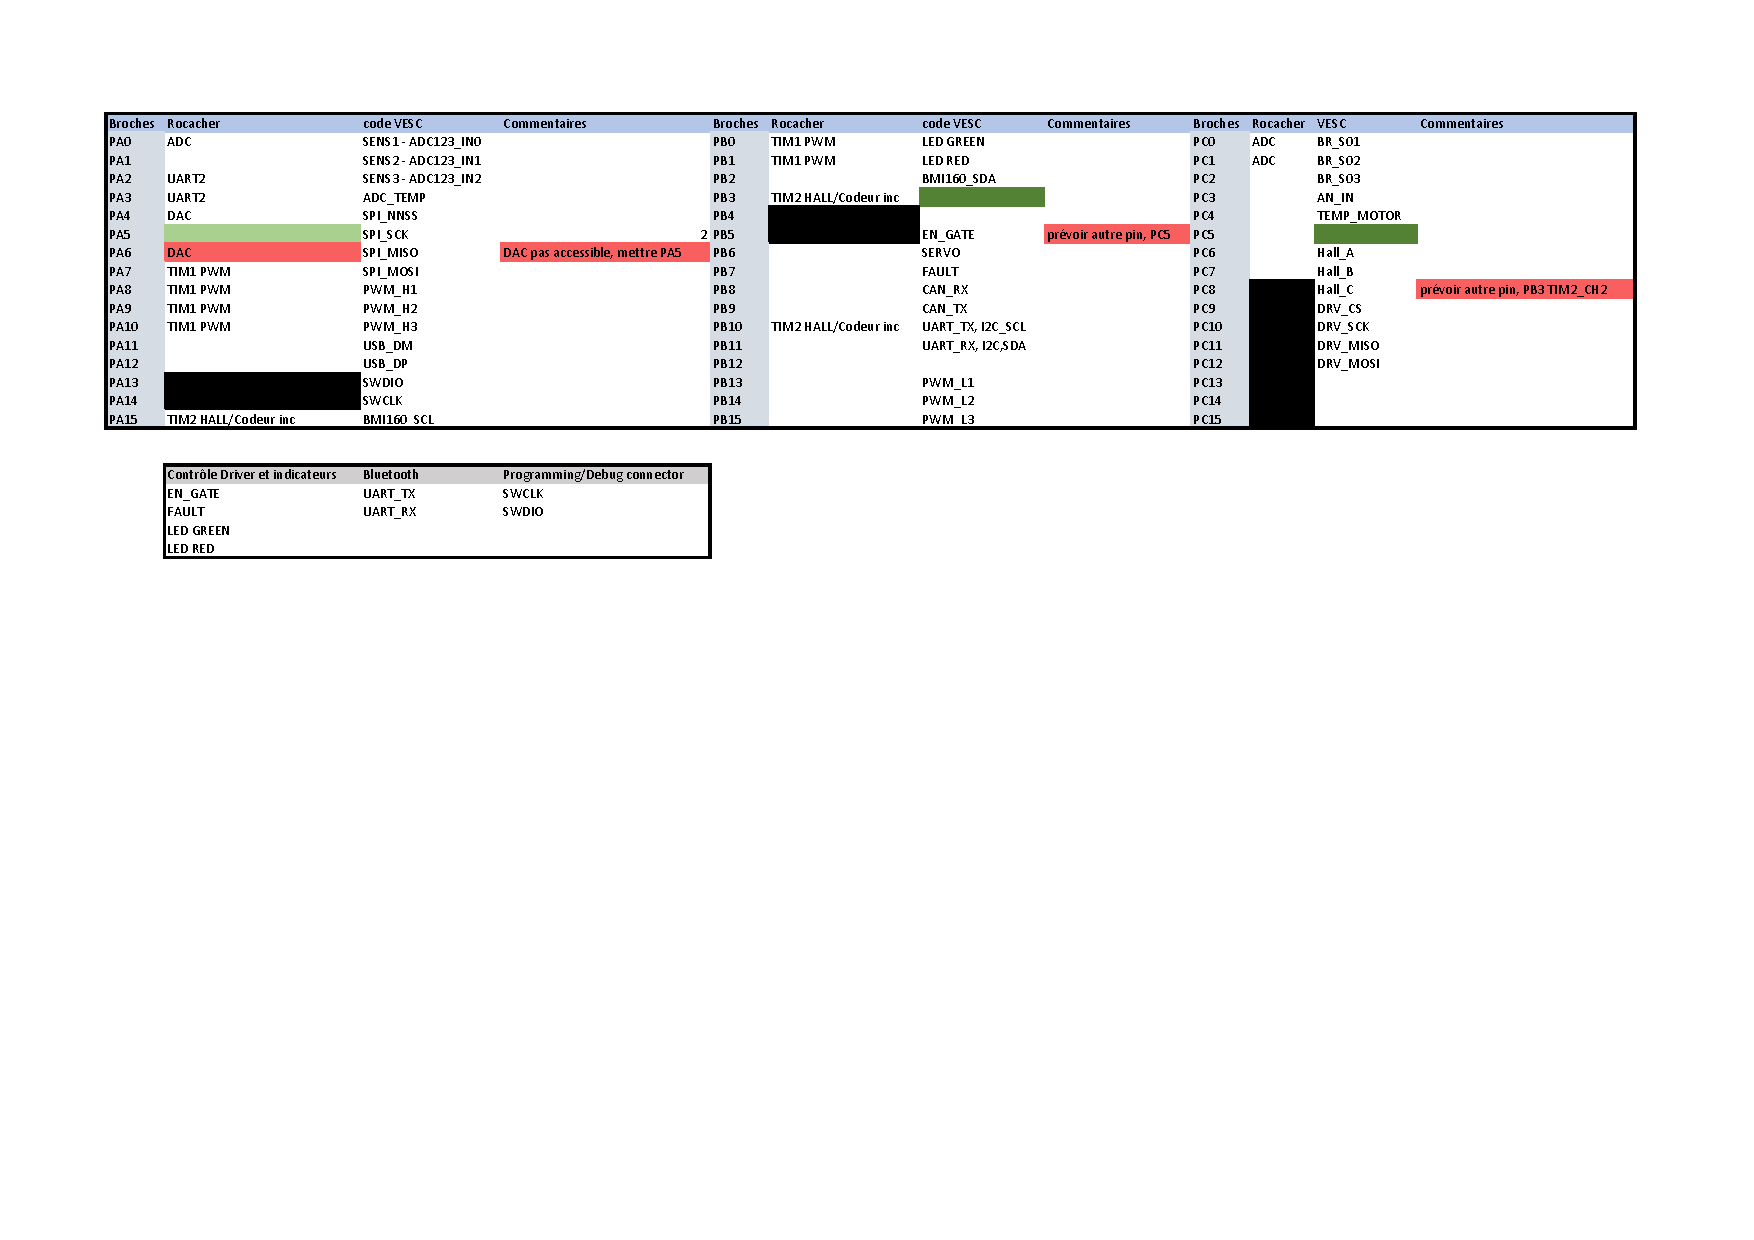
\includegraphics[width=\linewidth]{Figures/CompatibiliteL4F4.pdf}
    \caption{Comparison of F405 and L476 pin configurations}
    
\end{figure}

The first conflict concerned the SPI\_MISO signal on pin PA6. In the original STM32F405 design, this pin is used for SPI communication related to current sensing. On the STM32L476 tile, the same pin is associated with a DAC output, creating a functional conflict. To solve this issue, the SPI communication line was remapped to PA5 on the L476, which offers a compatible alternate function.

The second issue concerned the EN\_GATE signal. In the original design, this signal was connected to PB5 on the STM32F405. However, this pin is not accessible on the L476 tile. The signal was therefore moved to PC5, configured as a standard GPIO output.

Finally, Hall sensor C was originally connected to PC8 (TIM8) on the STM32F405. Since this pin is not available on the tile connector, the Hall sensor input was reassigned to PB3 using the TIM2\_CH2 alternate function, which preserves the input capture capability required for Hall sensor decoding.

All other important functions remained compatible between the two microcontrollers, including PWM generation, complementary PWM outputs, encoder inputs, UART, USB, and CAN communication. Some differences between the ADC peripherals of the STM32F405 and STM32L476 still remain and will require firmware adaptations in future work.

\subsection{Schematic Design and KiCad Implementation}

The original Cheap FOCer-2 schematic was modified in KiCad in order to replace the integrated STM32F405 microcontroller with connectors for the Rocacher STM32L476 tile. The objective was to make the control part more modular and easier to replace without modifying the power stage of the board.

The main modifications performed on the schematic were:
\begin{itemize}
    \item Removal of the STM32F405 and its associated passive components.
    \item Addition of two 20-pin headers for the L476 tile connection.
    \item Re-routing of PWM, ADC, USB, and communication signals toward the headers.
\end{itemize}

Special attention was given to the routing of critical control signals, especially the PWM outputs used for motor commutation and the analogue signals used for current sensing.

After the modifications, the schematic was verified using the KiCad Electrical Rule Check (ERC). No electrical errors were detected during this verification step, which validated the consistency of the schematic before starting the PCB routing phase.

\subsection{Routing Challenges and Current Status}

After validating the schematic, the PCB routing phase was started in KiCad. The original Cheap FOCer-2 board uses a very compact layout with dense routing around the STM32F405 microcontroller and the power stage. Integrating connectors for a removable STM32L476 tile introduced several additional routing constraints.

One of the main difficulties was maintaining proper signal routing while keeping enough space for the tile connectors and preserving the integrity of the control signals. Particular attention had to be given to the PWM signals, current sensing traces, and power connections.

Several issues were encountered during the routing process:
\begin{itemize}
    \item Some connector footprints associated with the tile did not appear correctly after importing the schematic into the PCB layout.
    \item The routing of high-current paths, especially the battery and motor phase connections, become more complex due to the additional connectors and required extra vias.
    \item Some Decoupling capacitors had to be repositioned, which could potentially affect switching noise and power
     supply stability.
\end{itemize}

At the current stage of the project, the schematic has been validated and the PCB layout is still under development. Once the routing is completed, the board will be manufactured and tested using the VESC firmware adapted for the STM32L476 tile.

\section{Hardware-Based Six-Step Commutation Controller}
\label{sec:sixstep}

The basis of this section is the replacement of components who are highly complex, technical and/or are dependant on global supply chains to manufacture. An additional goal is, as for the preceding section, to make a repairable, reliable and manufacturable circuit, this time using these more basic components, based on open-source principles. The controller needs to be performant enough to drive one of the two electric motors used on the LaMAD (La Manufacture Autonome Décentralisée) bicycle cargo trailer.\cite{noauthor_ddf-39_nodate}

\subsection{Constraints}
The electric motors used are supplied using 36/48 Volts at 1000 W. This means that the six-step chopper transistors need to be able to supply up to 28 Amperes of current. This is a lot, considering our restrictions. Additionally, the heat will need to be managed, which may be an even bigger challenge than the current.

\subsection{Semiconductor facilities in Occitanie}
The most challenging part of this section is the replacement of semiconductor parts, as these are the most complicated parts to manufacture. Luckily, the city in which the team is located, Toulouse, offers possibilities in semiconductor manufacturing. This may not be a complete list, but the following were identified:

\begin{enumerate}
	\item ST Microelectronics Labège-Innopôle (formerly Exagan, formerly CEA-Leti) 
	\item LAAS-CNRS (Laboratoire d'Analyse et d'Architecture des Systèmes - Centre National des Recherches Scientifiques) semiconductor lab
	\item AIME (Atelier Interuniversitaire de Micro-nano Électronique) on-campus at INSA Toulouse
\end{enumerate}

ST Microelectronics at Labège designs and manufactures gallium nitride transistors under the commercial designation STPOWER PowerGaN, this confirmed by a colleague who visited the plant and engineering teams in late 2022, Etienne Gadefait. Gallium nitride transistors are great for high speed power electronics % ref https://www.st.com/en/power-transistors/powergan.html
but this is a very recent technology, and none of the big material players in GaN are European, let alone French or Occitanian (US, China, Japan and India are predominant). % ref https://us.metoree.com/categories/7137/
 Because of this and very high costs, we chose to consider this a supply chain-constrained technology, which could not be relied on in a non-global future, and we moved on to other options.
 
The LAAS semiconductor lab was deemed less reachable and more technologically advanced than the AIME semiconductor lab, as we were told they mostly did research on carbon nanotubes and other fancy semiconductor materials. We therefore chose not to contact the LAAS, and 

The AIME is a small research lab located on our campus. Their capabilities and projects were not publicly available, so we decided to contact them. We met two researchers Mr. Tan and Mr. Lincelles to enquire about the manufacturability of certain components, and eventual costs. The AIME specialises in logic circuits, and has not developed any power components at least a decade. Therefore, the research teams have not maintained any know-how in power semiconductors. However, they were very interested in developing this field in their lab, and came with a proposal to start, based on their existing knowledge. Here are some of AIME's capabilities and prices:

\begin{table}[htbp]
	\caption{AIME capabilities}
	\label{tab:AIME_capabilities}
	\centering
	\begin{tabular}{lcc}
		\toprule
		\textbf{Proposal or capability} & \textbf{Value} & \textbf{Price, if relevant} \\
		\midrule
		Silicon wafer & 2'' ($\sim$50mm) & 10 € \\
		Epitaxial "fancy" wafer & 2'' ($\sim$50mm) & 100-200 €   \\
		AIME-made lithography mask &  10µm canal width & 300 € \\
		Lab rental & 1 day & $\sim$2000 € \\
		Transistor canal width & $\sim$1 µm \\
		Drain-source on resistance & 1 k\textOmega \\
		\bottomrule
	\end{tabular}
\end{table}

The proposed project was based on their logic transistors, scaled up not in size, but in number. As seen in the table above, one of their small logic transistors has a resistance of:

\begin{equation}
	R_{DS_{on}} \approx 1\ k\Omega
\end{equation}

As we need a transistor capable of passing 28 Amperes of current, this resistance is unacceptable. Therefore, they proposed to put a great number of transistors in parallel to reduce $R_{DS_{on}}$, on a big surface to better distribute and dissipate the heat (the heat calculations were not made). We can also note here that AIME does not have packaging technology to dissipate high head loads, which could be resolved using external specialist companies (expensive) or making a very thermally efficient transistor. The current also makes the attachment of wires more complicated, as the general relation (not taking into consideration the skin effect in larger diameters) they gave me gives:

\begin{equation}
	1\ \frac{mA}{\mu m\ diameter} \Rightarrow diameter =  2,8 cm
\end{equation}

Which is extremely unrealistic for a small component and needs to be investigated further. The second problem is the voltage, as the small signal transistors they have are made for lower voltages. Therefore, we needed a thicker MOSFET with a thicker n- drift layer between the drain and source to prevent breakdown, which results in us needing a fancy and expensive epitaxial wafer instead of a cheap one. This results in another problem, an even higher Drain-source on resistance $R_{DS_{on}}$, multiplying the already great number of transistors by a good factor. At the end, this is the project they proposed:

\begin{table}[htbp]
\caption{The project proposed by the AIME}
\label{tab:AIME_project}
\centering
\begin{tabular}{lcc}
\toprule
\textbf{Proposal or capability} & \textbf{Value} & \textbf{Price, if relevant} \\
\midrule
Transistor count & $\sim$400 000 & \\
Die size & 1-2 cm$^2$ & \\
Wafer & 2'' ($\sim$50mm) epitaxial & 100-200 €  \\
Dies per wafer & 1 & 100-200 € per die \\
Lab rental & subsidised &  reason: academia  \\
Masks needed & 4 & 1200 € \\
Dies per set of masks & $>$ 1000 dies & \\
\bottomrule
\end{tabular}
\end{table}

These costs are much larger than what we have for this project, but are not insurmountable for a department like the GEI. This project also needs a lot of time or more people to be made, more than what we have at our disposal. The researchers were very interested in collaborating on such a project in the future, and considered it very strongly as a replacement for the current AIME project for the 5th year PTP Energie students at INSA Toulouse (currently a CO2 sensor), with GEI's backing and funding. 

The complexity of manufacturing power transistors made us go for the strategy of choosing readily available and cheap components.


\subsection{Replacing an IC}

Replacing the IC of a motor controller requires using traditional logic gates. This approach can be done in several methods. The AIME would easily be able to produce such a circuit at a relatively low cost, but this is neither easily accessible nor repairable. We therefore needed to use another form of logic gates. The simplest form of gates are diode gates, which use two diodes to make either an AND or OR-gate. They cannot make NOT-gates, which need a CMOS-cell (two transistors). We continued by simulating this in LTSpice XVII, based on Mr. Rocacher's circuits. This circuit ended up needing 4 AND-gates, 2 OR-gates and 1 NOT-gate (CMOS cell) per phase, with additional transistors to compensate for voltage lost at the diodes, as well as one additional OR-gate. The total would be like this :

\begin{table}[htbp]
	\caption{Minimum number of diodes and transistors needed}
	\label{tab:decompte}
	\centering
	\begin{tabular}{lccc}
		\toprule
		\textbf{Gate} & Number of gates & \textbf{Number of diodes} & \textbf{Number of transistors} \\
		\midrule
		AND & 12  & 24 & 0 \\
		OR & 7 & 14 & 0 \\
		NOT & 3 & 0 & 6\\
		\bottomrule
		Total & & 38 & 6
	\end{tabular}
\end{table}

This is a considerable number of diodes and transistors, but would make the circuit easily repairable and replaceable.

\section{Software and Connectivity}

\subsection{BLE Compatibility With the VESC}

\subsubsection{First Experiment}
VESC-controllers are not necessarily equipped with Bluetooth-modules by default. Often, it is necessary to add a BLE-module. A standard HC-05 bluetooth-module compatible with Arduino is a great way to send and receive bluetooth-packets from a host, e.g. a mobile phone, via a bridge translating the bluetooth packets to the UART protocol. This could be demonstrated using a ESP8622's standard library with said module, by letting us send characters from one device to another.

\subsubsection{HC-05 and the VESC}
By flashing the VESC firmware on a discovery-card and connecting the HC-05 module to the PB10 and PB11-pins, which are the Rx and Tx-pins for the STM32F4xx chip, we discovered that the setup for the bluetooth module was not available in the VESC tool. The inherent BLE capabilities is an important limitation to consider when designing a VESC system. We learned therefore that the HC-05 is not originally adapted for BLE. The need for a bridge also adds on complexity and cost, in the form of extra components and another device to maintain the code of. For the future, choosing a bluetooth module supporting BLE will be the easiest solution. Preferably a module fitting the communication connector on the cheap FOCer project \cite{shamansystems_cheap-focer-2firmware_nodate} could facilitate the relevancy of the PCB project with a microcontroller.

\subsubsection{BLE Vulnerability}
Bluetooth could be a vulnerability to a VESC if it is to be used as a controller in real-time, as the controller could be jammed. Our test with the Flipper Zero shows the disfunctionnality of Bluetooth with different use cases. We experienced with the jamming of a bluetooth speaker that the music completely stopped. It could also be investigated how the connection to the VESC could be modified using the VESC tool. We will touch more on the accessibility of the code within the VESC tool sooner.

\subsection{Setup of BT-connection with VESC}
The setup consisted of a main PC/controller, HC-05 Bluetooth module, ESP8266 µ-controller, STM32 Discovery µ-controller, PC with VESC-tool as well as a \textit{FlipperZero}. Our plan of action consisted of flashing the Discovery-card with code for then to read this code via UART to the ESP8266 which was connected to the BT-module. The BT-module would then send packets to the PC. This PC would then act as read/write to read the code having been flashed on the Discovery. Full-band jamming would then be achieved by the implementation of the \textit{FlipperZero} disrupting any transfer of code from PC1 to PC2.The \textit{FlipperZero} was equipped with the firmware \textit{DarkFlippers/unleashed-firmware}\cite{noauthor_darkflippersunleashed-firmware_2026} with the addition of an NRF-jammer from \textit{huuck/FlipperZeroNRFJammer} \cite{cirlig_huuckflipperzeronrfjammer_2026}.

\newpage

\begin{figure}[!h]
    \centering 

\begin{tikzpicture}

% PC_ESP
\node[
    draw,
    rectangle,
    minimum width=1.5cm,
    minimum height=1.5cm
] (PC1) at (2.5,-0.5)
{
   
\includegraphics[width=1.5cm]{Figures/PC_STOCK.jpg}
};
\node[above=2mm of PC1] {PC1 ready to r/w};


% HC05
\node[
    draw,
    rectangle,
    minimum width=1.5cm,
    minimum height=1.5cm
] (HC05) at (-0.3,-2.6)
{
   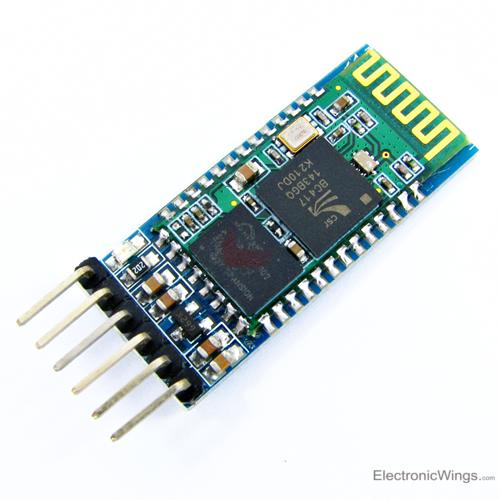
\includegraphics[width=1.5cm]{Figures/HC-05_Bluetooth_Module.jpg}
};
\node[above=1mm of HC05] {HC-05};

\node[
    draw,
    rectangle,
    minimum width=1.5cm,
    minimum height=1.5cm
] (ESP) at (-0.3,-5)
{
    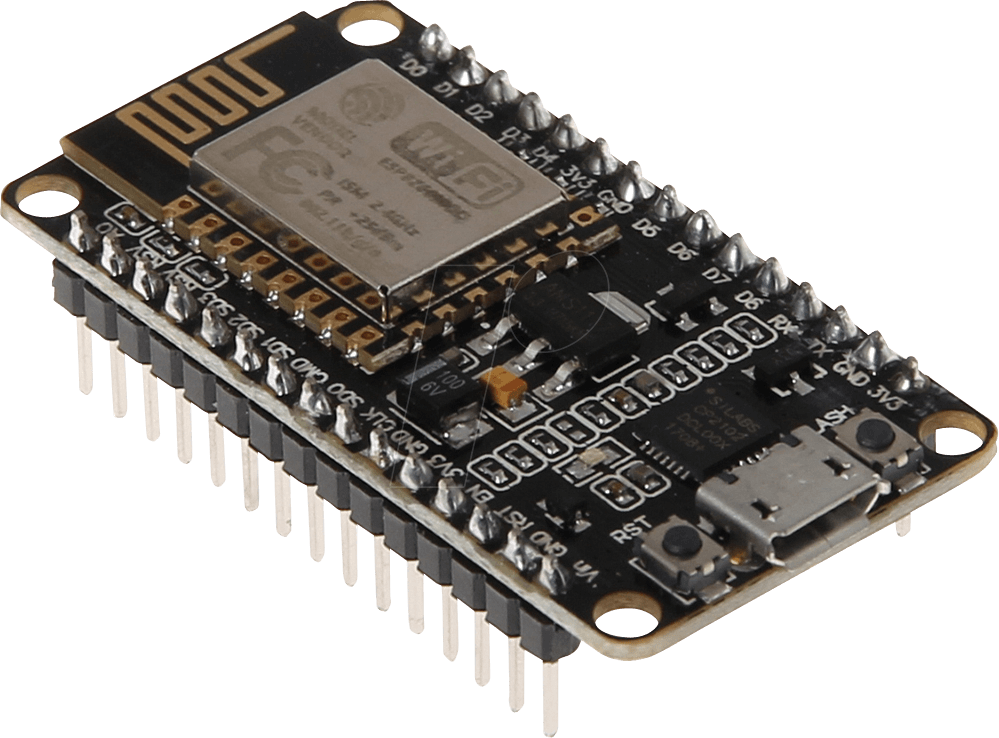
\includegraphics[width=1.5cm]{Figures/ESP8266.png}
};
\node[below=1mm of ESP] {ESP8266};

\node[
    draw,
    rectangle,
    minimum width=1.5cm,
    minimum height=1.5cm
] (PC2) at (-3.6,-2.6)
{
    
\includegraphics[width=1.5cm]{Figures/PC_STOCK.jpg}
};
\node[above=1mm of PC2] {PC2 with VESC-tool};

\node[
    draw,
    rectangle,
    minimum width=1.5cm,
    minimum height=1.5cm
] (Disc) at (-3.6,-5)
{
   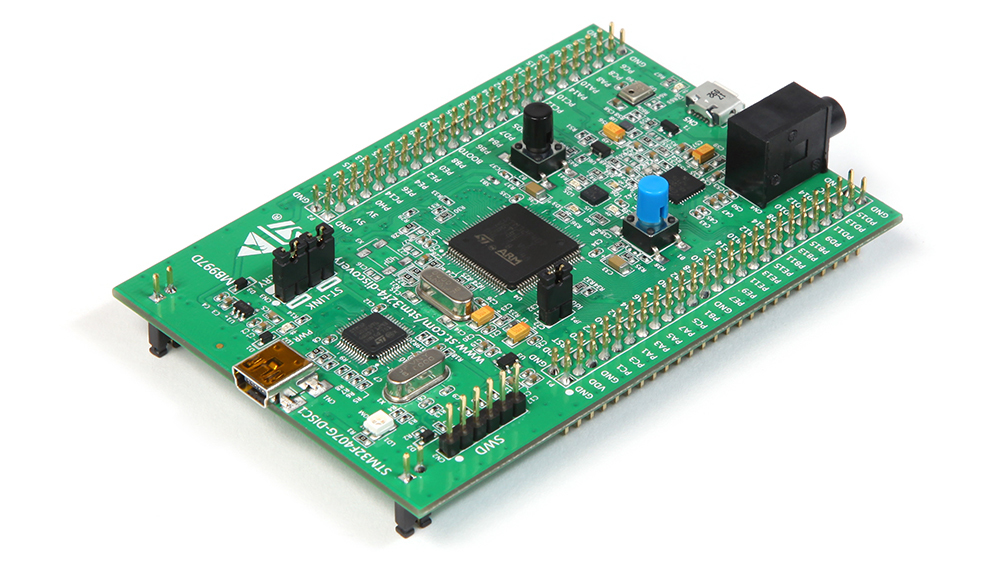
\includegraphics[width=1.5cm]{Figures/STM32_Discovery.jpg}
};
\node[below=1mm of Disc] {STM32 Discovery};

\node[
    draw,
    rectangle,
    minimum width=1.5cm,
    minimum height=1.5cm
] (F0) at (-1.5,0)
{
    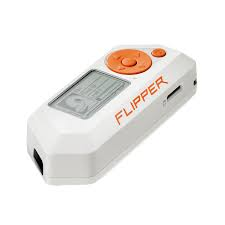
\includegraphics[width=1.5cm]{Figures/F0.jpeg}
};
\node[above=1mm of F0] {FlipperZero};

% Arrow between boxes
%\draw[decorate, decoration={snake}] (box1) -- (box2);
\draw[->, thick] (HC05) -- (ESP);
\draw[<->, decorate, decoration={snake}] (PC1) -- node[below right]{BT-connectivity} (HC05);
\draw[->] (HC05) -- node[left]{UART} (ESP);
\draw[<->] (HC05) -- node[right]{Tx $\leftrightarrow$ Rx} (ESP);

\draw[<->] (ESP) -- node[below]{UART} (Disc);
\draw[<->] (ESP) -- node[above]{Tx $\leftrightarrow$ Rx} (Disc);

\draw[<->] (Disc) -- node[left]{USB} (PC2);

\draw[->, decorate, decoration={snake}] (F0) -- node[above=3mm]{Jamming} (1.25,-1.5);
\

\end{tikzpicture}
 \caption{Setup of BT-connection wih VESC.} 
  \label{fig:BT} 

\end{figure}



\subsection{Code integrity}
\subsubsection{Context}
As the project is open source, and the code is freely accessible, there should be no reason to hide the code. It could however be reasonable to protect the code from changes which could hurt other people. Changing following parameters should at least come with a disclaimer and clearly state the dangers possible by proceeding with said changes. We have in mind the maximum speed permitted and the power available to the motors.

\subsubsection{LispBM extraction}
We caught word that the lisp code for the VESC used by Maillon mobility was easy to extract. By building an older firmware with the Maillon mobility software, we observed this by going to the lispBM tab and clicking read. It's up to the MAD if they would like to reinforce this mechanism. A modification on a parameter and then clicking upload allowed us to easily change the speed limit. This could bring up a public danger. This raises questions on the use of the MAD's equipment, as it's used in a day-to-day traffic environment. 

\subsubsection{LispBM Code}
When we flashed newer firmware from the project made by Benjamin Vedder\cite{b1}, we also observed some difficulties in uploading the lispBM script taken from the one on firmware version 6.06. This could indicate that there needs to be further maintenance of the code in order to get the software up to date. This needs to be documented better for someone  to continue the project. This could be a good investment for the MAD.

This documentation could be as simple as referencing the relevant parts of the lispBM documentation. \cite{b2}

\subsubsection{Proposed Solution}
This risk could be patched by developing a VESC application for the VESC controller or using a binary. This is a solution which is less open source, but defends well against malicious intent.The application could be created using C and use an algorithm known by the MAD in order to secure the access to someone to change the parameters only if they are MAD certified personnel. This encryption would preferably be reduced to the most essential settings in order to align with what our impression of the philosophy of the MAD would be.


\subsection{VESC Compiling}
As mentioned, we have been able to compile the VESC tool and the VESC firmware. This firmware has been put onto an STM32F4xx Discovery card. This card uses the same chip as the aforementioned ``Cheap FOCer'' project. The thought was that using something with the same chip would facilitate the switch from the discovery card to a PCB with the same target.

However, this choice posed several obstacles for our progress on the topic of cybersecurity. We will nonetheless summarise what we have learned for you and propose some additional work for the future. The challenges we encountered were the following: The lack of bluetooth capabilities. We did not have a module with BLE either. We had access to a HC-05 module, but that only allows for a normal Bluetooth version 2.0 protocol and would require further work on a bridge to UART by using an esp8622 that we had as well. We propose that the next group has access to a VESC controller from the beginning, as well as a motor we could control. This could be in cooperation with the MAD, as the MAD could propose some models they're interested in.

We also found that the information on the VESC is scattered around the internet. The resources is also sometimes based on a Debian-based Linux system which adds more work for someone using another distribution of Linux. This could hinder the implementation facility for new users. We struggled particularly with the Qt packages for positioning and game pad. We would therefore recommend the use of a Debian-based Linux system for the computer working with the VESC for the MAD associates.





\section{Dynamic Modelling and Control of the Bicycle-Cargo System}

\subsection{Dynamic System Modelling} 

The studied system consists of a bicycle towing a cargo cart through a rigid mechanical linkage. This link is only used for steering guidance and does not contribute to the traction force. The main objective is to ensure that the rider perceives minimal additional effort, such that the overall behaviour remains similar to riding a standard bicycle. 

From a control perspective, the rider provides a reference motion in terms of speed and position, while the cargo cart is expected to follow this reference with minimal delay. The position error between the bicycle and the cargo cart is computed using a distance sensor, which provides feedback relative to an equilibrium state. 

The cargo cart is modelled as the plant of the system. Its rotational dynamics are described using the fundamental equation of rotational motion: 

\begin{equation*}
\sum \tau = J_{\Delta} \times \dot{\omega} 
\end{equation*} 
where $\tau$ is the total torque applied to the system, $J_{\Delta}$ is the equivalent moment of inertia, and $\omega$ is the angular velocity. 

The total torque is composed of the motor torque $\tau_m$ and a friction torque modelled as: 

\begin{equation*} 
\tau_f = -f \times \omega 
\end{equation*} 
where $f$ is the viscous friction coefficient. 

The resulting dynamic equation becomes: 

\begin{equation*} 
J_{\Delta} \dot{\omega} = \tau_m - f \omega 
\end{equation*} 

In the Laplace domain, this leads to: 
\begin{equation*} 
\omega(s) = \frac{\tau_m(s)}{J_{\Delta} s + f} 
\end{equation*} 

Since the linear velocity is related to angular velocity by the wheel radius $R$, we obtain: 

\begin{equation*} 
v(s) = R \times \omega(s) 
\end{equation*} 

Thus, the transfer function between motor torque and linear velocity is: 
\begin{equation*} 
\frac{v(s)}{\tau_m(s)} = \frac{R}{J_{\Delta} s + f} 
\end{equation*} 


\subsection{PI-Based Control Strategy} 
\label{subsec:Simulink_model}
Based on this model, a Simulink representation of the system was developed. The controlled system includes a feedback loop using a PI (Proportional-Integral) controller in order to regulate the position error between the bicycle and the cargo cart. 

Since the reference input is a ramp signal (representing the bicycle position over time), an integral action is required to ensure zero steady-state error and accurate tracking of the reference trajectory. 

The closed-loop Simulink model of the system is shown in Fig.~\ref{fig:simulink-closedloop}. 

The control error is defined as the difference between a desired relative position and the measured displacement between the bicycle and the cargo cart:
\begin{equation*}
    e(t) = e_{\text{ref}} - (x_{\text{bike}} - x_{\text{cart}})
\end{equation*}
where $e_{\text{ref}} = \SI{-0.5}{\meter}$ represents the desired equilibrium offset between both systems.

\begin{figure}[!h]

    \centering 
    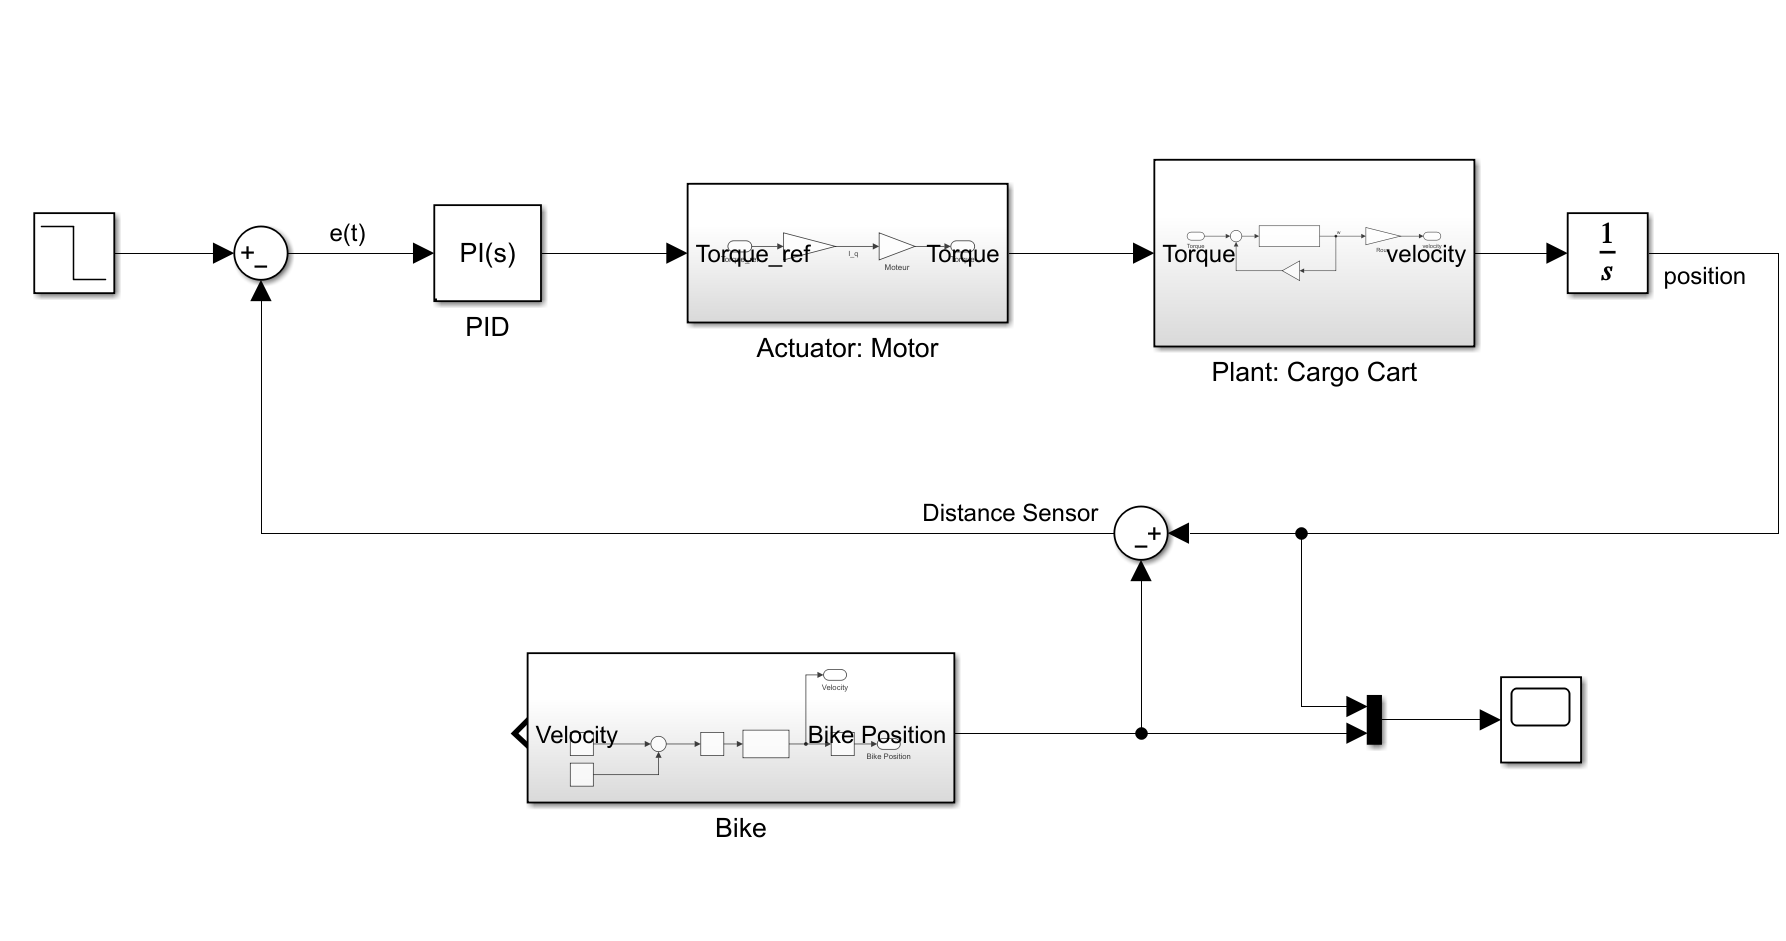
\includegraphics[width=\linewidth]{./Figures/sys_dyn_matlab.png} 
    \caption{Closed-loop model of the bicycle-cargo system with PI control.} 
    \label{fig:simulink-closedloop} 

\end{figure} 


\subsection{Control Architecture Exploration}
Beyond the standard PI control structure simulated in the previous sections, this project explores a more sophisticated control law: the Cascaded Loop Architecture. This approach is envisioned as a high-level software enhancement to meet the robustness and safety requirements inherent to electric cargo mobility. This means that our control law includes two feedback loops that use two different physical parameters. 

The selected cascaded structure is a well-established industry standard, particularly in high-performance motion control and robotics. Similar architectures are widely employed in Automated Guided Vehicles (AGVs) and platooning systems, where a “follower” unit must synchronize its dynamics with a “leader” unit through precise feedback loops.

The proposed approach decomposes the complex task of “cart following” into manageable sub-tasks by nesting control loops: 
\begin{itemize}
    \item Outer loop: Position control layer.
    Using a linear encoder or distance sensor mounted on the trailer’s hitch, the system measures the relative displacement (error) between the bicycle and the cargo cart. This error is processed by a Proportional (P) Controller. The primary goal of this stage is to translate physical distance into a target velocity setpoint. By saturating the output of this loop, we can prevent the cargo cart from ever exceeding the bicycle’s speed, thereby ensuring it never “pushes” the cyclist. 

    \item Inner loop: Velocity control layer.
    The velocity setpoint generated by the outer loop is fed into this internal layer, the inner loop is responsible for commanding the motor torque directly to compensate for immediate mechanical disturbances. Because this loop operates at a higher frequency, it can reject disturbances such as sudden changes in rolling resistance or friction, before they significantly impact the overall position error. 
\end{itemize}

\begin{figure}[!h]

    \centering 
    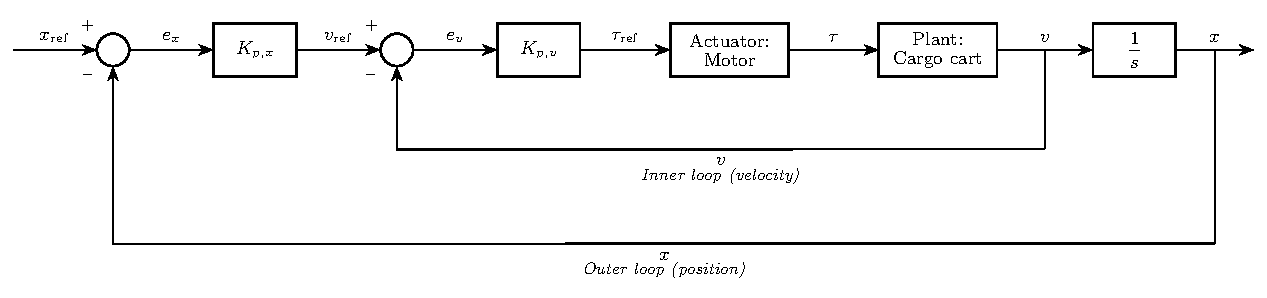
\includegraphics[width=\linewidth]{./Figures/Schema_Autom_PIR.pdf} 
    \caption{Cascaded control architecture for the bicycle-cargo system.} 
    \label{fig:cascaded-loop} 

\end{figure}

Fig.~\ref{fig:cascaded-loop} illustrates the cascade architecture for the dynamics of the cargo cart. In this scheme, $x_{\text{ref}}$ denotes the desired position of the bicycle, whereas $x$ represents the measured position of the cargo cart.

An outer Proportional Controller $K_{p,x}$ converts the position error $e_x = x_{\text{ref}} - x$ into a velocity reference $v_{\text{ref}}$, which serves as the set-point for the inner loop.
The inner Proportional Controller $K_{p,v}$ then transforms the velocity error $e_v = v_{\text{ref}} - v$ into a torque reference $\tau_{\text{ref}}$.
This command is processed by the motor/actuator block, which delivers the actual torque $\tau$.
The model of the plant maps this torque to velocity $v$, and the integrator $1/s$ reconstructs the position $x$.

The adoption of a cascaded loop architecture offers decisive advantages but comes with disadvantages. This precision introduces increased complexity: the multiplication of tuning parameters and the requirement for high-resolution feedback sensors, such as encoders, raise hardware costs and must come with high-performance software. These technical constraints represent a significant challenge and may raise other issues.






% Fin
\section{Results}

\subsection{FOC Controller Validation}
	
	\subsubsection{Current Status Summary}
	
	Table~\ref{tab:foc_status} summarizes the current status of the FOC 
	controller development.
	
	\begin{table}[htbp]
	\caption{FOC controller development status}
	\label{tab:foc_status}
	\centering
	\begin{tabular}{l c}
	\toprule
	\textbf{Task} & \textbf{Status} \\
	\midrule
	VESC firmware compilation & Completed \\
	Pin compatibility (F405 / L476) & Completed \\
	Schematic design (KiCad) & Completed \\
	ERC validation & Completed \\
	PCB routing & In progress \\
	Tile footprint correction & In progress \\
	Board manufacturing & Planned \\
	Hardware testing & Planned \\
	\bottomrule
	\end{tabular}
	\end{table}

\subsection{Bicycle-Cargo System Control Results}

\subsubsection{Simulation Results}
The closed-loop Simulink model presented in the subsection~\ref{subsec:Simulink_model} was used to evaluate the performance of the proposed PI-based (Proportional-Integral) control strategy.

Figure~\ref{fig:tracking-error} shows the evolution of the tracking error between the bicycle and the cargo cart during simulation. The response exhibits an initial transient phase followed by a progressive convergence toward the desired equilibrium position, demonstrating stable closed-loop behaviour and satisfactory tracking performance.
\begin{figure}[!h]
    \centering 
    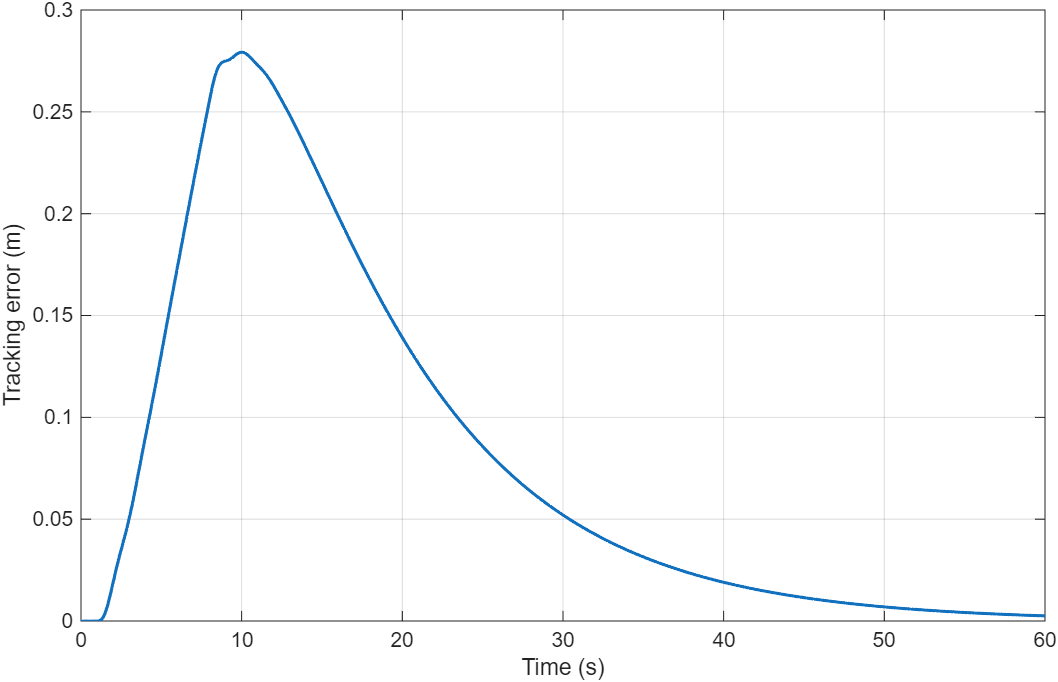
\includegraphics[width=\linewidth]{./Figures/error_fig.png} 
    \caption{Position tracking error between bicycle and cargo cart.} 
    \label{fig:tracking-error} 
\end{figure} 

\subsubsection{Experimental Load Characterization}
Experimental tests were conducted on flat terrain in order to evaluate the influence of mechanical load on the motor current consumption of the cargo cart system. The system was powered using a \SI{48}{\volt} battery pack.

Current measurements were acquired using an Analog Discovery 2 connected to a computer running the WaveForms software environment. A current clamp probe was used to measure the motor current, and the signals were sampled at \SI{1}{\kilo\hertz}.

During each test, the throttle command was set to its maximum value in order to produce the highest possible acceleration. Once the maximum speed was reached, the motor current naturally decreased and stabilised as the motor only compensated for rolling resistance and friction effects.

Three loading conditions were investigated corresponding approximately to one, two, and three passengers inside the cargo cart. The motor current measured during these experiments is shown in Fig.~\ref{fig:motor-currents}.

\begin{figure}[!h]
    \centering 
    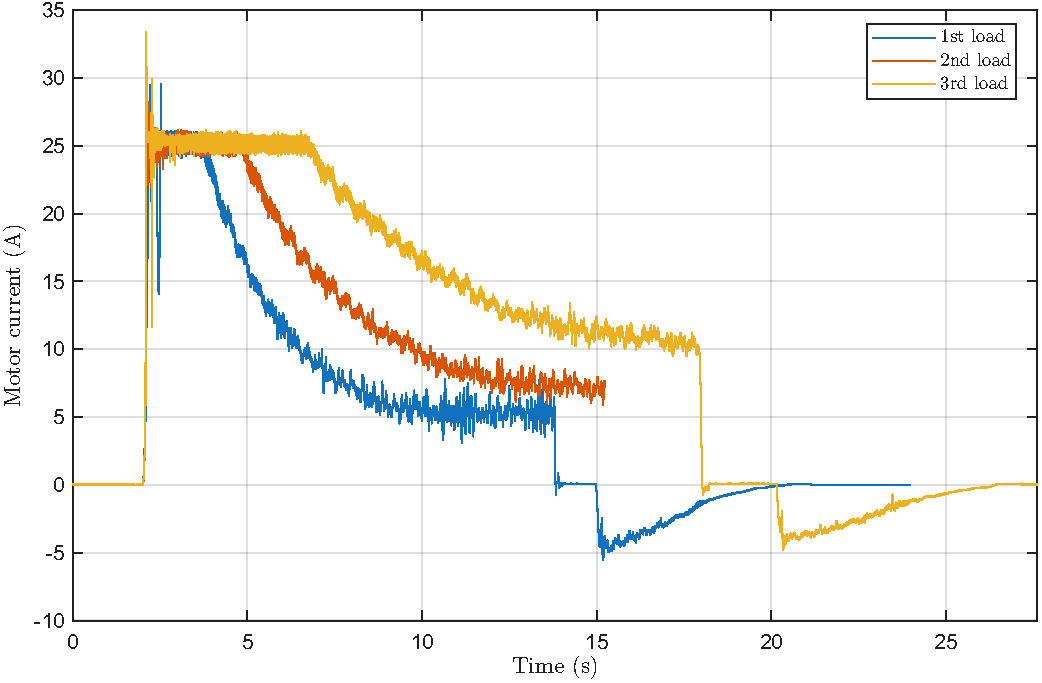
\includegraphics[width=\linewidth]{./Figures/Motor_currents.pdf} 
    \caption{Measured motor current under three loading conditions.} 
    \label{fig:motor-currents} 
\end{figure} 

The results show a significant current peak during the acceleration phase, reaching the controller limit of approximately \SI{25}{\ampere}. After this transient phase, the current decreases and converges toward a lower steady-state value corresponding mainly to friction and resistive force compensation.

As expected, higher loading conditions resulted in higher steady-state current consumption, indicating an increase in the required motor torque. In addition, the duration during which the current remained close to the maximum controller limit also increased with heavier loads, reflecting the longer acceleration time required to reach steady-state operation.
These variations are mainly attributed to terrain irregularities, throttle response fluctuations, and limitations associated with the measurement setup and current probe acquisition chain.

However, due to the absence of direct velocity measurements during the experiments, only qualitative observations could be extracted from these tests. Consequently, a precise estimation of dynamic friction parameters and energy efficiency could not be achieved.

\subsection{FOC Controller Validation}

\subsubsection{Current Status Summary}

Table~\ref{tab:foc_status} summarizes the current status of the FOC controller development.

\begin{table}[htbp]
\caption{FOC controller development status}
\label{tab:foc_status}
\centering
\begin{tabular}{l c}
\toprule
\textbf{Task} & \textbf{Status} \\
\midrule
VESC firmware compilation & Completed \\
Pin compatibility (F405 / L476) & Completed \\
Schematic design (KiCad) & Completed \\
ERC validation & Completed \\
PCB routing & In progress \\
Tile footprint correction & In progress \\
Board manufacturing & Planned \\
Hardware testing & Planned \\
\bottomrule
\end{tabular}
\end{table}



\section{Discussion}
This project could be seen as an introduction to the VESC project for someone who don't know about it from beforehand, the challenges the new users face during setup, as well as a demand for clear expectations concerning documentation on the subject. The project the MAD is leading should probably not be a fork of the project, as the project is still in development.

As a final note, this proved to be a project which could easily be developed into several different projects in different fields. Some projects could be continued later on as a different PIR subject, other could be proposed to later years in different specialisations like TLS-SEC, ESPE. Our thoughts on the following projects that could be 

The fabrication line for electronics is globalised. This is okay in a stable world, but it could be a problem in a world full of instability, be it war, blockages, or tariffs. The idea of opening a specialisation in cooperation with AIME came up as an idea.

For TLS-SEC the subject could be the design for a fitting mechanism to restrict certain privileges to certified personnel that could be used in the C programming language. Later down the line we could also see the possibility to analyse the Bluetooth frames in order to manipulate them in order to change important parameters.

The continuation on the PCB could be a subject fitting an ESPE specialisation.

The proposition of and supply of a VESC system to play with and troubleshoot could be a good rule of thumb, which allows for a quicker start and gives among other things an idea of the budget and the supply line used by a entity in the sector. Proposing a visit could also be one way to familiarise students with the association.

What should be a clear conclusion from our test with the jammer is that a controller based on Bluetooth alone should be avoided when possible and practical. Examples where this could be relevant include electric skateboards, as cables could impose a tripping hazard. There, an encapsulation of an encrypted control frame could be an thought. 





\section{Perspectives and Future Work}
Based on the results obtained and the limitations identified during this project, several directions for future work are proposed.

\subsection{Hardware Completion and Testing}
The VESC-based FOC PCB requires routing completion and prototype manufacturing. Once fabricated, the board must be tested under real operating conditions (varying loads, road profiles, and battery voltage).

\subsection{Control Strategy Enhancement}
Future work includes the implementation and comparison of the PI controller and the cascaded control structure on the cargo cart, in order to evaluate their performance under different conditions (load variations, road profiles, etc.).

In addition, the lack of direct velocity measurements limited the ability to fully characterise the system dynamics. Adding a speed measurement or improving state estimation would allow a more complete analysis of the model.




\section{Conclusion/Summary}

%\begin{figure}[htbp]
%%\centerline{\includegraphics{fig1.png}}
%caption{Example of a figure caption.}
%\label{fig}
%\end{figure}

%Figure Labels: Use 8 point Times New Roman for Figure labels. Use words 
%rather than symbols or abbreviations when writing Figure axis labels to 
%avoid confusing the reader. As an example, write the quantity 
%``Magnetization'', or ``Magnetization, M'', not just ``M''. If including 
%units in the label, present them within parentheses. Do not label axes only 
%with units. In the example, write ``Magnetization (A/m)'' or ``Magnetization 
%\{A[m(1)]\}'', not just ``A/m''. Do not label axes with a ratio of 
%quantities and units. For example, write ``Temperature (K)'', not 
%``Temperature/K''.

\section*{Acknowledgment}
The authors would like to thank Pascal Acco and Thierry Rocacher for their continuous technical guidance and support throughout this project. Their expertise in power electronics, embedded systems, and PCB design was invaluable.

We also thank La Manufacture Autonome Décentralisée (LaMAD) for providing the use case, the technical requirements, and the cargo bike platform used for validation.

Finally, we acknowledge the INSA Toulouse GEI department for providing access to laboratory facilities, measurement equipment, and the necessary components for prototyping.

This work was carried out as part of the 4th-year research project (PIR) at INSA Toulouse.




\section*{Statement on AI Usage}
The authors acknowledge the use of generative AI tools during this project, both for the development work and for writing this paper.

AI was used as a helper in several parts of the project. This includes support for understanding and structuring technical ideas, and giving suggestions during the development of different subsystems. It was also used to help with writing, rephrasing, and improving clarity in the report.

However, all final decisions, implementations, and validations were done by the authors. The AI outputs were always checked, corrected when needed, and adapted based on reliable technical sources and our own experiments and understanding of the system.

We consider AI as a useful tool to speed up thinking and writing, but not as a source of final technical truth. Everything related to design choices, analysis, and results was verified and fully controlled by the authors.

The use of AI tools in this work follows the IEEE guidelines for generative AI usage in publications.






%Please number citations consecutively within brackets \cite{b1}. The 
%sentence punctuation follows the bracket \cite{b2}. Refer simply to the reference 
%number, as in \cite{b3}---do not use ``Ref. \cite{b3}'' or ``reference \cite{b3}'' except at 
%the beginning of a sentence: ``Reference \cite{b3} was the first $\ldots$''

\bibliographystyle{IEEEtran}
\bibliography{PIR_MadMax3}


\end{document}
